% ==============================================================================
\chapter{Active edge sensors}
\label{ch:ActiveEdgeSensors}
%==============================================================================    

%% --------------------------------------------- %%
\section{Introduction}

Thin n-in-p planar sensors produced by Advacam~\cite{AdvacamRef} are
bump bonded to the Timepix3 readout chips ($55\,\micron$ pixel pitch)
and studied in test beams and simulations.  Active-edge sensors allow
for seamless tiling of pixel matrices in large areas of a vertex
detector by depleting them to their physical edge. This allows for
high coverage without creating overlaps between the pixel matrices and
therefore reduces the material. Planar n-in-p pixelated sensors with
active edge using a Deep Reactive Ion Etching (DRIE) process have been
produced. This process consists of extending the backside implantation
to the edge. Figure~\ref{fig:activeedge} illustrates a cross section
of an active-edge sensor with and without guard ring. Since the
back-side voltage is extended to the edge of the sensor, the gradient
of potential between the edge and the last pixel can be very high and
could lead to a breakdown of the sensor. A guard ring consists of an
n-implant with a metallic contact on top of it surrounding the pixel
matrix close to the edge and thereby smoothening the potential
transition between the edge and the neighbouring pixels. The potential
of the guard ring can be floating or grounded by connecting it to the
ground of the readout ASIC. Timepix3 ASICs provide an extra row of
bumped pixels allowing to connect the guard ring to ground.


\begin{figure}[htbp]
  \begin{center}
    \begin{tikzpicture}
      \node[anchor=south west,inner sep=0] (image) at
      (0,0){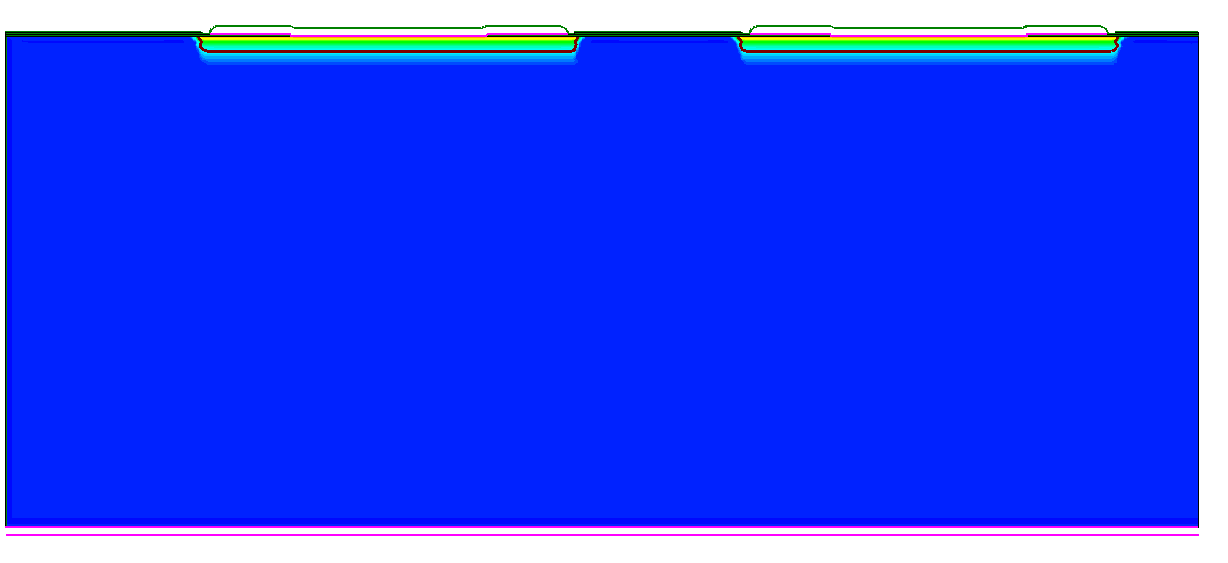
\includegraphics[width=.6\textwidth]{figures/ActiveEdge/schematic.png}};
      \begin{scope}[x={(image.south east)},y={(image.north west)}]
        \draw[-, dashed, line width=.7pt, color=white](0.1, 0.05) -- (0.1, 0.92);
        \draw[-, dashed, line width=.7pt, color=white](0.54, 0.05) -- (0.54, 0.92);
        \draw[<->, line width=.7pt, color=black](0.01, 0.97) -- (0.16, 0.97); % edge width
        
        \node[above, color=black] at (0.05, 0.97) {edge (20 \micron)};
        
        \draw[<->, line width=.4pt, color=black](0.17, 0.97) -- (0.47, 0.97); % n-implant
        \node[above, color=black] at (0.33, 0.97) {n-implant (36 \micron)};
        \node[above, color=white] at (0.3, 0.5) {p-substrate};
        \draw[<->, line width=.4pt, color=black](0.54, 0.0) -- (0.98, 0.0); % pixel width
        \node[below, color=black] at (0.75, 0.0) {pixel (55 \micron)};
        
        \draw[-, line width=3pt, color=violet](0.0, 0.05) -- (0.98, 0.05); % p+ backside contact
        \node[below, color=violet] at (0.15, 0.0) {p+ backside contact};
        \draw[-, line width=3pt, color=violet](0.0, 0.045) -- (0.0, 0.93); % p+ active-edge contact
        \node[left, color=violet, rotate=90] at (-0.05, 0.7) {p+ active edge};
        \node[left, color=white, rotate=90] at (0.08, 0.7) {final pixel edge};

        % \draw[help lines,xstep=.1,ystep=.1] (0, 0) grid (1,1);
        % \foreach \x in {0,1,...,9} { \node [anchor=north] at (\x/10,0) {0.\x}; }
        % \foreach \y in {0,1,...,9} { \node [anchor=east] at (0,\y/10) {0.\y}; }

      \end{scope}
    \end{tikzpicture}
    \caption{Schematic showing the cross section of a sensor with
      $20\,\micron$ active-edge technology. The pixel edges considered
      in the analysis are indicated with dashed lines.}
    \label{fig:activeedge}
  \end{center}
\end{figure}


\begin{table}[htbp]
  \centering
  \caption{Advacam active-edge n-in-p planar pixel sensor assemblies. The edge distance is defined by the distance between the last pixel implant and the physical sensor edge.}
  \label{tab:activeEdgeAssembliesList}
  \begin{tabular}{lccc}
    \toprule
    Assembly & Thickness [\micron] & Edge distance [\micron] & ID \\
    \midrule
    20-NGR  & 50 & 20 & W19\_G7 \\
    23-FGR & 50 & 23 & W19\_F7 \\ \hline
    28-GNDGR & 50 & 28 & W19\_L8 \\
    55-GNDGR & 50 & 55 &W19\_C7 \\
    55-GNDGR-100 & 100 & 55 & W5\_E2  \\ \hline
    55-GNDGR-150 & 150 & 55 & W5\_F1 \\
    \bottomrule
  \end{tabular}
\end{table}

The IV measurement is shown in Figure~\ref{fig:IVmeasurements}.

\begin{figure}[htbp]
  \centering
  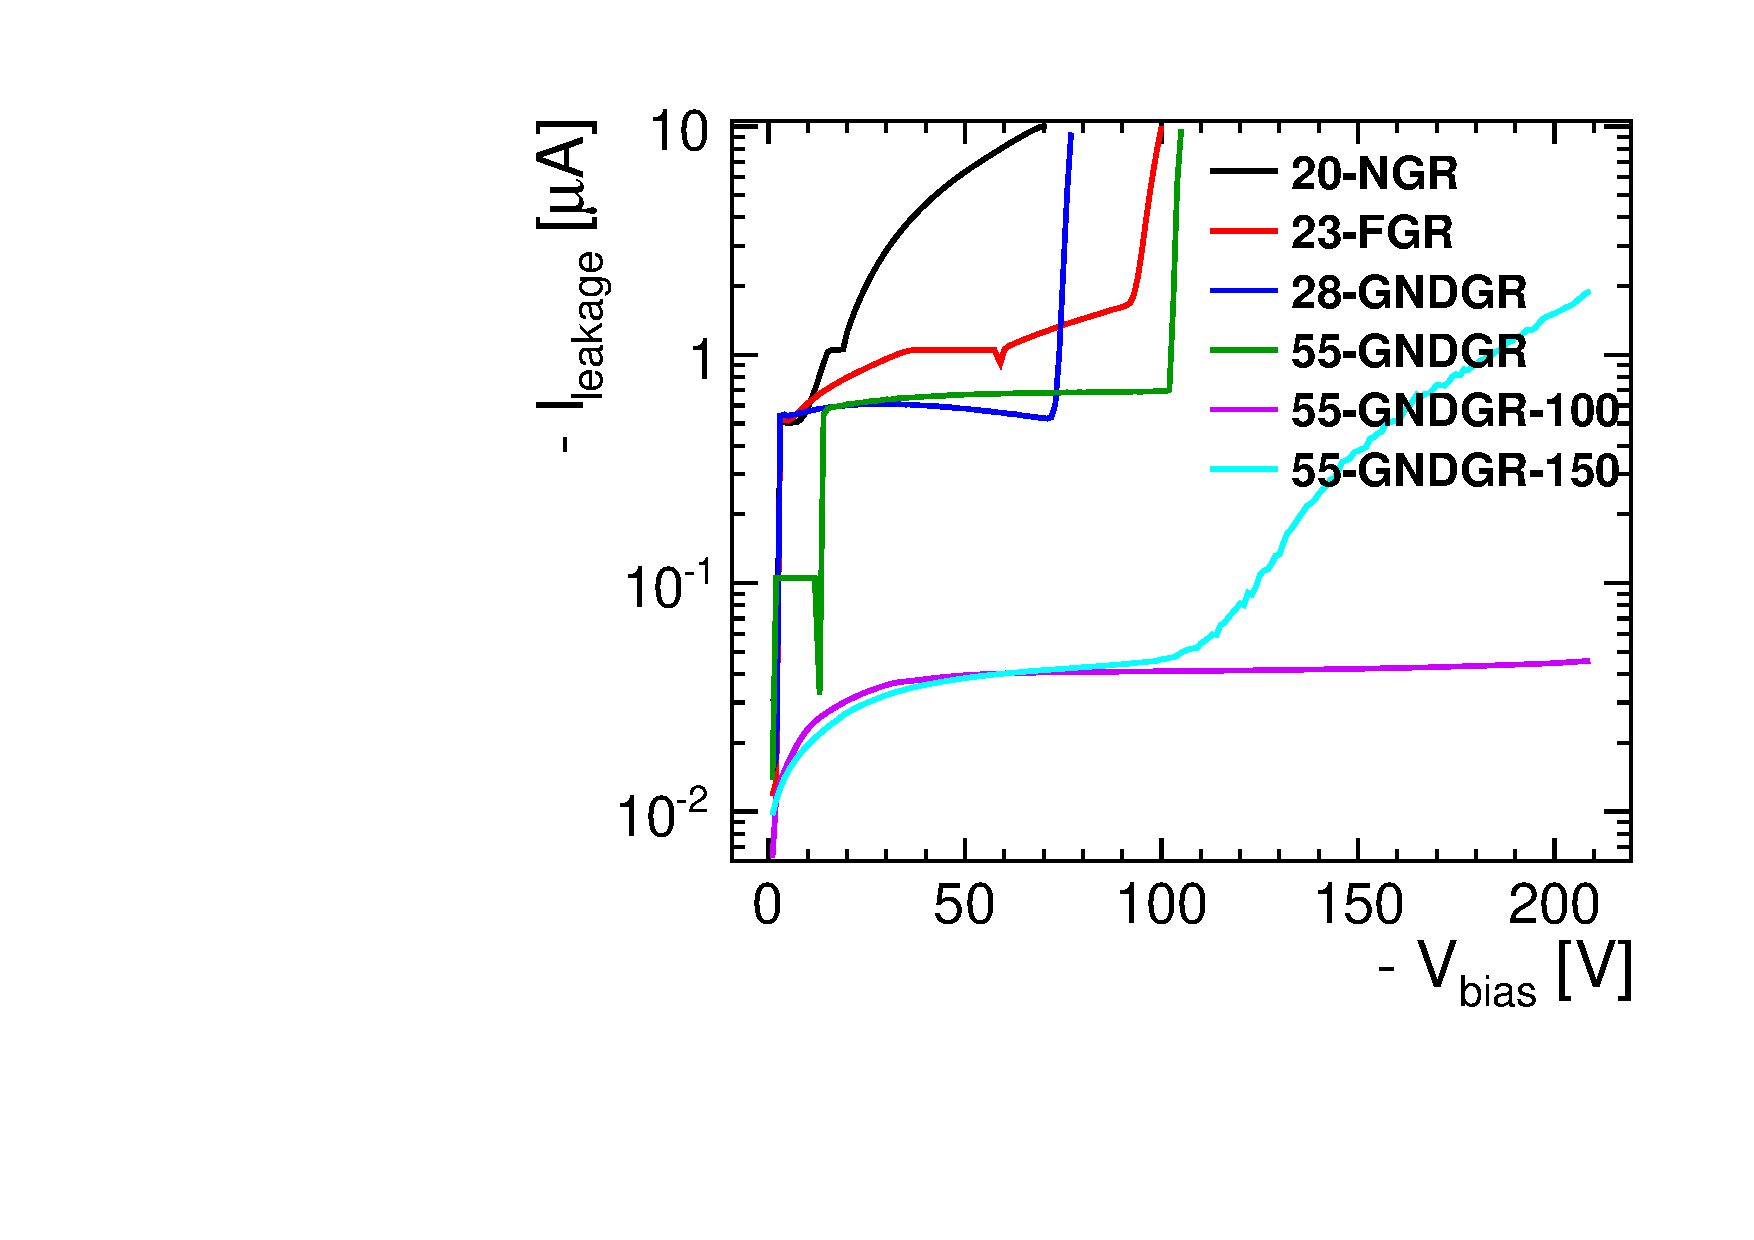
\includegraphics[width=0.7\textwidth]{figures/ActiveEdge/IVCurve.pdf}
  \caption{IV measurements for the assemblies listed in Table~\ref{tab:activeEdgeAssembliesList}.}
  \label{fig:IVmeasurements}
\end{figure}

\subsection{Sensor geometries}
The layers in the geometry description are defined in
Figure~\ref{fig:PixelLayout} and explained in
Table~\ref{tab:PixelStackDimensions}.

\begin{figure}[htbp]
  \centering
  \begin{minipage}[t]{.4\textwidth}
    \centering
    \vspace{0pt}
    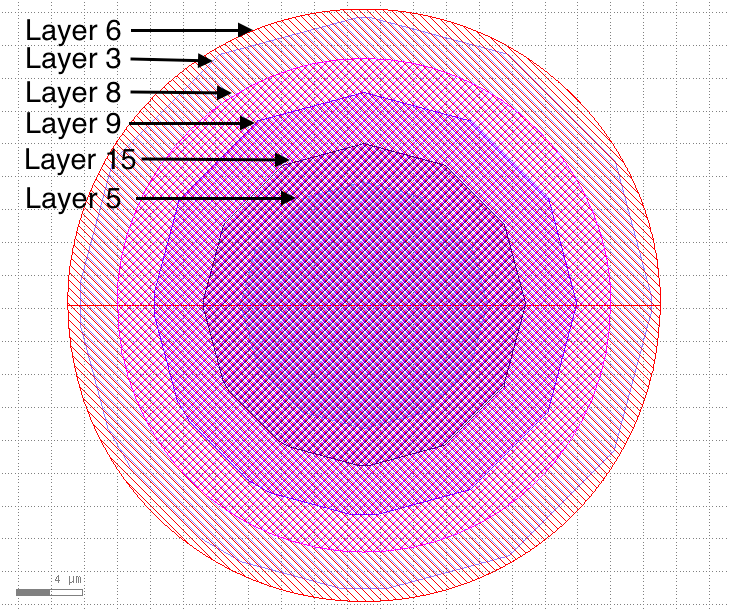
\includegraphics[width=0.95\textwidth]{figures/ActiveEdge/pixelLayout_withLayers.png}
    \caption{}
    \label{fig:PixelLayout}
  \end{minipage}
  \hfill
  \begin{minipage}[t]{.56\textwidth}
    \centering
    \vspace{0pt}
    \captionof{table}{Layers in the sensor from the gds file
      (Picture from 23-FGR).}
    \label{tab:PixelStackDimensions}
    \begin{tabular}{l c c}
      \toprule
      Layer number & Layer \\
      \midrule
      6 & metal\\
      3 & - \\
      8 & implant \\
      9 & UBM (for thin film lift off metal) (??) \\
      15 & passivation \\
      5 & contact to connect Al to Si \\
      \bottomrule
    \end{tabular}
  \end{minipage}
\end{figure}

Table~\ref{tab:DimensionsForAssemblies} summarises the dimensions of
the implants for the sensors. The edge width is the distance between
the last pixel implant to the physical edge of the sensor. The metal
width is the diameter of the metal for the pixels. The doping width is
the diameter of the pixels implant. The contact width is the diameter
of the contact between silicon and the metal (where the oxide is
etched). The GR offset is the distance between the physical edge of
the sensor and the implant of the GR.

\begin{table}
  \centering
  \captionof{table}{The pixels and guard-ring dimensions for different assemblies}
  \label{tab:DimensionsForAssemblies}
  \begin{tabular}{l c c c c}
    \toprule
    & 20-NGR & 23-FGR & 28-GNDGR & 55-GNDGR \\
    \midrule
    Edge width [\micron] & 20 & 23 & 28 & 55 \\
    Metal width [\micron] & 40 & 36 & 36 & 40 \\
    Doping width [\micron] & 30 & 30 & 30 & 30 \\
    Contact width [\micron] & 15 & 15 & 15 & 15 \\
    GR offset [\micron] & - & 10 & 14.5 & 25 \\
    GR doping width [\micron] & - & 5 & 5 & 5 \\
    GR contact width [\micron] & - & 3 & 3 & 3 \\
    GR metal width [\micron] & - & 7 & 7 & 10 \\
    \bottomrule
  \end{tabular}
\end{table}






For the 50~\micron grounded GR, the dimensions of the pixels are
differente from above.
\captionof{table}{Layers and dimensions from the gds geometry
  (taken from Timepix 20um GR FLOAt and from Timepix 50~\micron grounded GR).}
\label{tab:PixelStackDimensions}
\begin{tabular}{l c c c}
  \toprule
  Layer number & Layer & Diameter (20 float) [\micron] & Diameter (50 GND) [\micron]\\
  \midrule
  6 & metal & 36 & 40 \\
  3 & - & 34.62 & 36 \\
  8 & implant & 30 & 30 \\
  9 & UBM & 25.6 & 25.6 \\
  15 & passivation & 19.5 & 19.5 \\
  5 & contact to connect Al to Si & 15 & 15 \\
  \bottomrule
\end{tabular}


\begin{figure}[htbp]
  \centering
  \begin{subfigure}[b]{0.33\textwidth}
    \centering
    \fbox{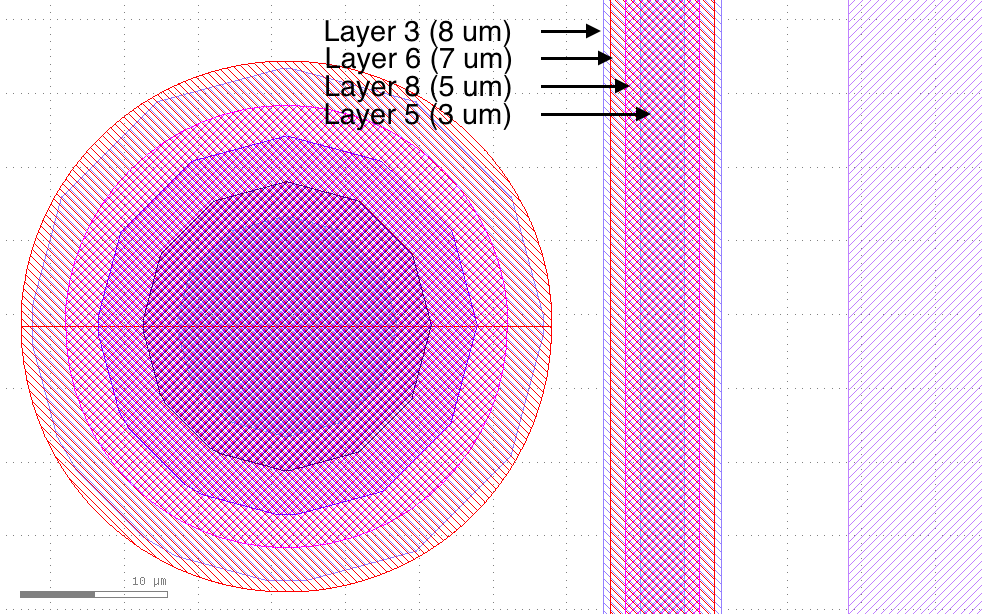
\includegraphics[width=0.95\textwidth]{figures/ActiveEdge/20umEdge_float_GR_withText.png}}
    \caption{20~\micron edge: Floating guard ring}
    \label{fig:GuardRingLayout_20_float_GR}
  \end{subfigure}\hfill
  \centering
  \begin{subfigure}[b]{0.33\textwidth}
    \centering
    \fbox{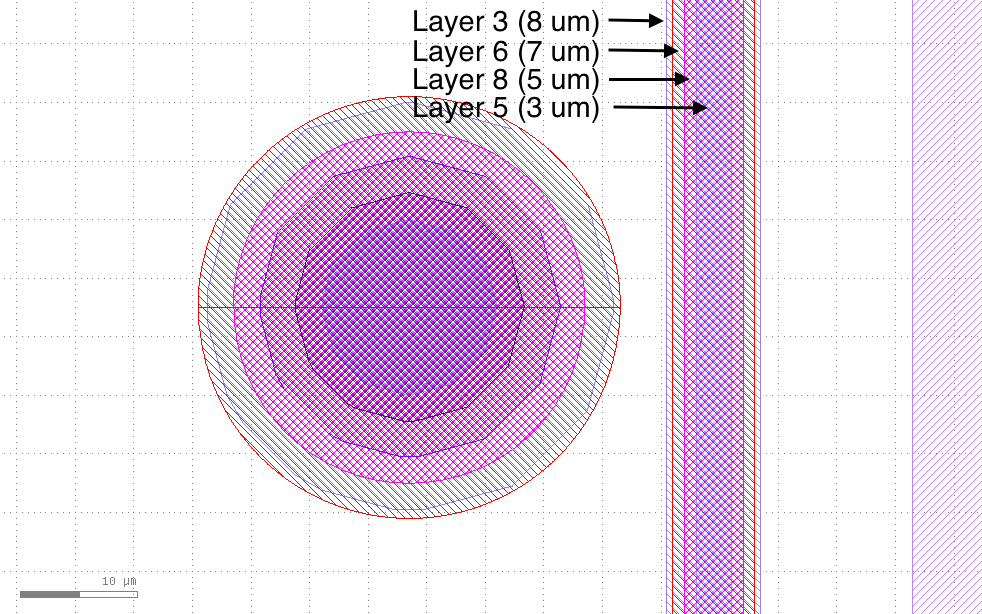
\includegraphics[width=0.95\textwidth]{figures/ActiveEdge/20umEdge_GND_GR_withText.png}}
    \caption{20~\micron edge: GND guard ring}
    \label{fig:GuardRingLayout_20_GND_GR}
  \end{subfigure}\hfill
  \centering
  \begin{subfigure}[b]{0.33\textwidth}
    \centering
    \fbox{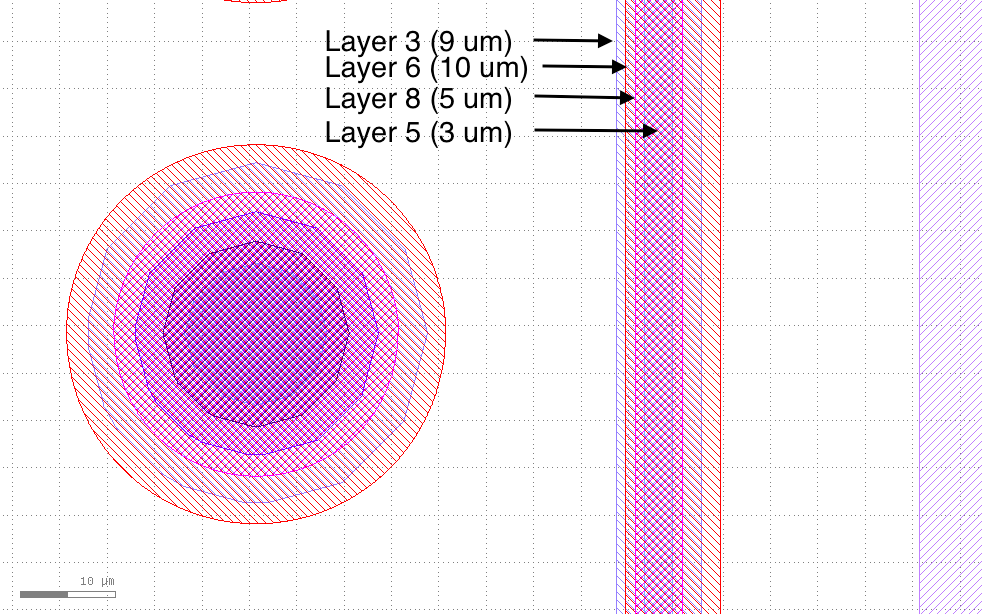
\includegraphics[width=0.95\textwidth]{figures/ActiveEdge/50umEdge_GND_GR_withText.png}}
    \caption{50~\micron edge: GND guard ring}
    \label{fig:GuardRingLayout_50_GND_GR}
  \end{subfigure}
  \label{fig:GuardRingLayout}
\end{figure}

\subsection{Test-beam analysis of the edge}
\begin{figure}[htbp]
  \begin{subfigure}[b]{0.5\linewidth}
    \centering
    \begin{tikzpicture}
      \node[anchor=south west,inner sep=0] (image) at (0,0) {
        \includegraphics[width=\linewidth, page=3]{figures/TestBeam/edge_bcp.pdf}};
    \end{tikzpicture}
    \caption{}
    \label{fig:}
  \end{subfigure}\hfill
  \begin{subfigure}[b]{0.5\linewidth}
    \centering
    \begin{tikzpicture}
      \node[anchor=south west,inner sep=0] (image) at 
      (0,0){\includegraphics[width=\textwidth, page=5]{figures/TestBeam/edge.pdf}};
    \end{tikzpicture}
    \caption{}
    \label{fig:}
  \end{subfigure}
  \caption{(a) Efficiency and (b) charge (TOT) collected as a function of the
    track position for the assembly 20-NGR.}
  \label{fig:20-NGR_eff_TOT}
\end{figure}


\begin{figure}[htbp]
  \begin{subfigure}[b]{0.5\linewidth}
    \centering
    \begin{tikzpicture}
      \node[anchor=south west,inner sep=0] (image) at (0,0)
      {\includegraphics[width=\textwidth, page=6]{figures/TestBeam/edge_bcp.pdf}};
    \end{tikzpicture}
    \caption{}
  \end{subfigure}\hfill
  \begin{subfigure}[b]{0.5\linewidth}
    \centering
    \begin{tikzpicture}
      \node[anchor=south west,inner sep=0] (image) at 
      (0,0){\includegraphics[width=\textwidth, page=8]{figures/TestBeam/edge.pdf}};
    \end{tikzpicture}
    \caption{}
    \label{fig:}
  \end{subfigure}
  \caption{(a) Efficiency and (b) charge (TOT) collected as a function of the
    track position for the assembly 23-FGR.}
  \label{fig:23-FGR_eff_TOT}
\end{figure}


\begin{figure}[htbp]
  \begin{subfigure}[b]{0.5\linewidth}
    \centering
    \begin{tikzpicture}
      \node[anchor=south west,inner sep=0] (image) at (0,0)
      {\includegraphics[width=\textwidth, page=9]{figures/TestBeam/edge_bcp.pdf}};
    \end{tikzpicture}
    \caption{}
  \end{subfigure}~
  \begin{subfigure}[b]{0.5\linewidth}
    \centering
    \begin{tikzpicture}
      \node[anchor=south west,inner sep=0] (image) at 
      (0,0){\includegraphics[width=\textwidth, page=11]{figures/TestBeam/edge.pdf}};
    \end{tikzpicture}
    \caption{}
  \end{subfigure}
  \caption{(a) Efficiency and (b) charge (TOT) collected as a function of the
    track position for the assembly 28-GNDGR.}
  \label{fig:28-GNDGR_eff_TOT}
\end{figure}


\begin{figure}[htbp]
  \begin{subfigure}[b]{0.5\linewidth}
    \centering
    \begin{tikzpicture}
      \node[anchor=south west,inner sep=0] (image) at (0,0)
      {\includegraphics[width=\textwidth, page=12]{figures/TestBeam/edge_bcp.pdf}};
    \end{tikzpicture}
    \caption{}
  \end{subfigure}\hfill
  \begin{subfigure}[b]{0.5\linewidth}
    \centering
    \begin{tikzpicture}
      \node[anchor=south west,inner sep=0] (image) at 
      (0,0){\includegraphics[width=\textwidth,
        page=14]{figures/TestBeam/edge.pdf}};
    \end{tikzpicture}
    \caption{}
  \end{subfigure}
  \caption{(a) Efficiency and (b) charge (TOT) collected as a function of the
    track position for the assembly 55-GNDGR.}
  \label{fig:55-GNDGR_eff_TOT}
\end{figure}

\begin{figure}[htbp]
  \begin{subfigure}[b]{0.5\linewidth}
    \centering
    \begin{tikzpicture}
      \node[anchor=south west,inner sep=0] (image) at (0,0)
      {\includegraphics[width=\textwidth, page=15]{figures/TestBeam/edge_bcp.pdf}};
    \end{tikzpicture}
    \caption{}
  \end{subfigure}\hfill
  \begin{subfigure}[b]{0.5\linewidth}
    \centering
    \begin{tikzpicture}
      \node[anchor=south west,inner sep=0] (image) at 
      (0,0){\includegraphics[width=\textwidth,
        page=17]{figures/TestBeam/edge.pdf}};
    \end{tikzpicture}
    \caption{}
  \end{subfigure}
  \caption{(a) Efficiency and (b) charge (TOT) collected as a function of the
    track position for the assembly 55-GNDGR-100.}
  \label{fig:55-GNDGR-100_eff_TOT}
\end{figure}


\begin{figure}[htbp]
  \begin{subfigure}[b]{0.5\linewidth}
    \centering
    \begin{tikzpicture}
      \node[anchor=south west,inner sep=0] (image) at (0,0)
      {\includegraphics[width=\textwidth, page=18]{figures/TestBeam/edge_bcp.pdf}};
    \end{tikzpicture}
    \caption{}
  \end{subfigure}\hfill
  \begin{subfigure}[b]{0.5\linewidth}
    \centering
    \begin{tikzpicture}
      \node[anchor=south west,inner sep=0] (image) at 
      (0,0){\includegraphics[width=\textwidth,
        page=20]{figures/TestBeam/edge.pdf}};
    \end{tikzpicture}
    \caption{}
  \end{subfigure}
  \caption{(a) Efficiency and (b) charge (TOT) collected as a function of the
    track position for the assembly 55-GNDGR-150.}
  \label{fig:55-GNDGR-150_eff_TOT}
\end{figure}

%% --------------------------------------------- %%
\newpage
\section{TCAD simulations}
\subsection{Process flow for the active-edge designs}

\begin{itemize}
\item Sprocess 1:
  \begin{enumerate}
  \item First the dimensions of the pixels, implants, contacts, metal
    layer are defined.
  \item The meshing is refined at the borders, the implants and also
    based on the concentration using an adaptive meshing using the
    \texttt{refinebox} command.
  \item The silicon region is then defined for the two pixels and the
    edge region and an extra silicon edge which will be etched (to make
    the process more realistic). The silicon is doped with borons (p-type material)
    with the initial resistivity of $\rho=10000 \Omega$cm ($4.41\times
    10^{11}\,\inversecmcubic$). 
  \item A layer of $0.2\,\micron$ thick of Oxide is deposited.
  \item A layer of $0.2\,\micron$ thick of Nitride is deposited.
  \item The silicon is then doped with borons with a concentration of
    $10^{12}\,\inversecmcubic$. From the bias scan of the $150\,\micron$ thick
    silicon, the depletion voltage was obtained at 16~V and confirms the
    doping concentration of the silicon. The implantation done is done
    at the energy of $180\,\kev$.
  \item The nitride is then etched at the positions where the
    implantation is going to be done. First the a mask is put on the
    positions where the Nitride is going to stay. Then the etching is
    done at the implantation positions. Phosphorus (n-type material) is
    implanted with a dose of $10^{15}\,\inversecmcubic$ with an energy
    of $120\,\kev$.
  \item The extra edge is etched to achieve the edge width wanted. First
    the Nitride layer is etched, then the Oxide and finally the silicon
    layer is etched.
  \item The sensor is then flipped and a layer of oxide is deposited on
    the backside with a thickness of $0.04\,\micron$. An implantation is
    done with Boron with a concentration of $10^{15}\,\inversecmcubic$
    with an energy of $60\,\kev$. Then the oxide is etched from the
    backside and the sensor is flipped again to the initial position.
  \end{enumerate}

\item Sprocess 2:
  \begin{enumerate}
  \item The oxide is then etched at the contact positions.
  \item A photoresist is deposited on the top of the sensor with a
thickness of $2\,\micron$.
  \item The meshing of the edge is then refined adaptively depending
on the concentration of the ions and for a thickness of $1\,\micron$.
  \item Borons are implanted to the edge with a concentration of
$10^{15}\,\inversecmcubic$, an energy of $60\,\kev$ and a title of
$15\degrees$C.
  \item The photoresist is then removed (\texttt{strip resist}).
  \item To activate the dopants, the sensor is annealed at a constant
temperature of $940\degrees$C during 240 minutes.
  \item The metal layer is deposited using Aluminium of thickness
$0.8\,\micron$.
  \item The sensor is then flipped and on the back-side, a layer of
aluminium with a thickness of $0.8\,\micron$ for the contact of the
high-voltage is deposited.
  \end{enumerate}
\end{itemize}

Masks limit the etching and the deposition to a certain range of
window and provide the possibility to imitate the lithographic
patterning.

The doping concentration for the different layouts is shown in
Figure~\ref{fig:TCAD_dopingConcentration}.

%% --------------------------------------------- %%
\subsection{Electric field distribution in simulations}
In silicon, the breakdown field occurs for electric field exceeding
$\sim3\cdot10^5$~\voltpercm. In active-edge sensors, since the
back-side implantation as well as the bias voltage are extended to the
edge of the sensor, the gradient of potential between the edge and the
last pixel can be very high. This could lead to a breakdown of the
sensor. In TCAD simulations, the electric field distribution for the
sensors operated at nominal conditions are shown in
\cref{fig:TCAD_Efield2D}. In any case, for the nominal conditions, the
breakdown electric field is never reached and in the laboratory
measurements, this can be seen through the measurement of the leakage
current as shown in \cref{fig:IVmeasurements}.

\begin{figure}[htbp]
  \centering
  \begin{subfigure}[b]{0.5\linewidth}
    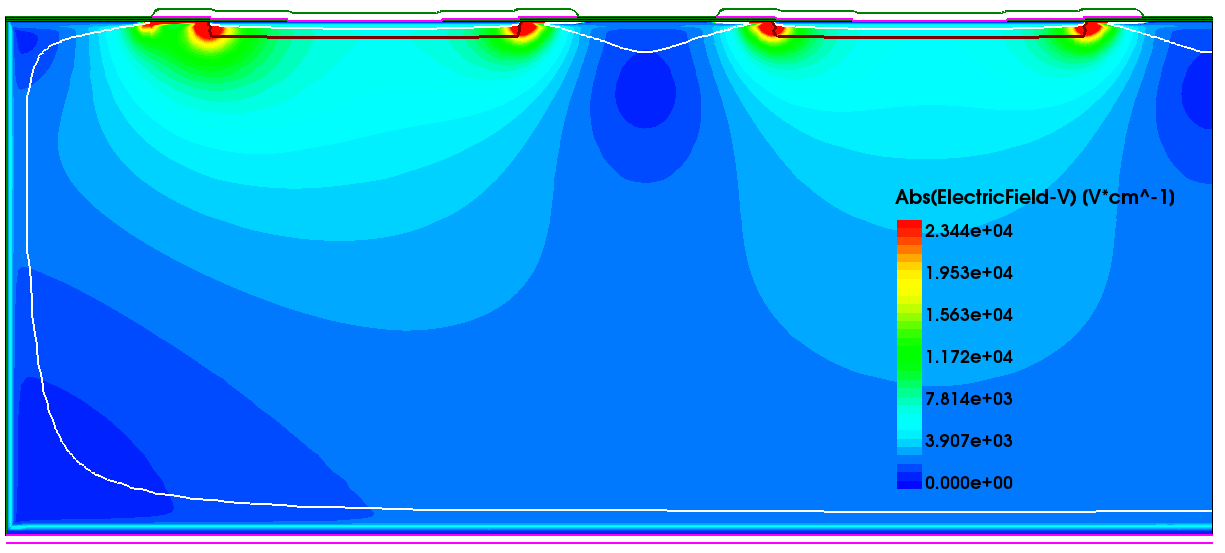
\includegraphics[width=\textwidth]{figures/ActiveEdge/Efield_20_NGR.png}
    \caption{20-NGR}
  \end{subfigure}\hfill
  \begin{subfigure}[b]{0.5\linewidth}
    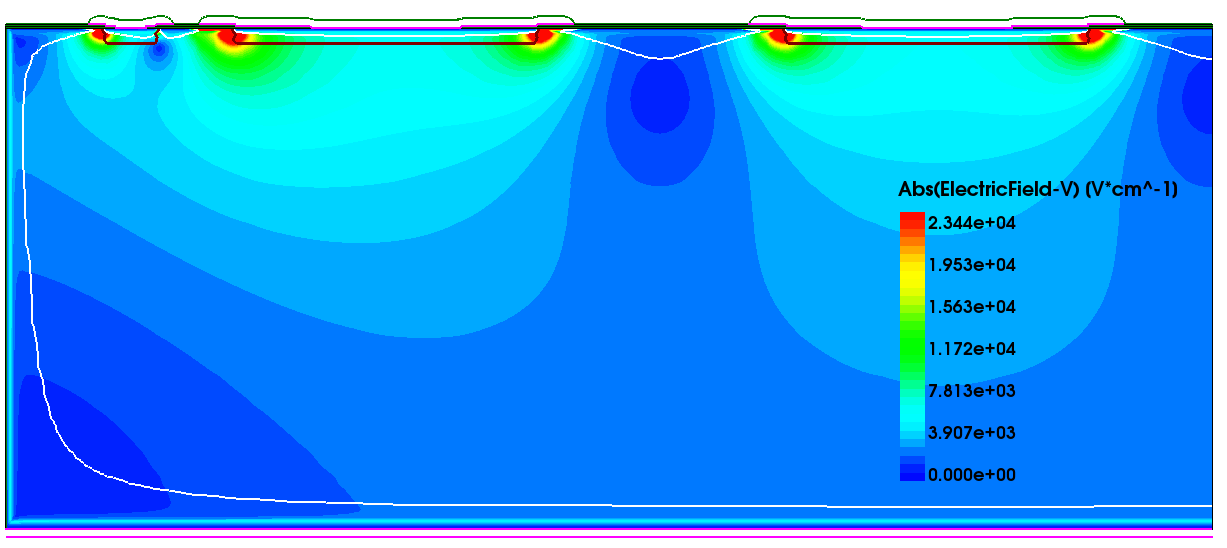
\includegraphics[width=\textwidth]{figures/ActiveEdge/Efield_23_FGR.png}
    \caption{23-FGR}
  \end{subfigure} \\
  \begin{subfigure}[b]{0.5\linewidth}
    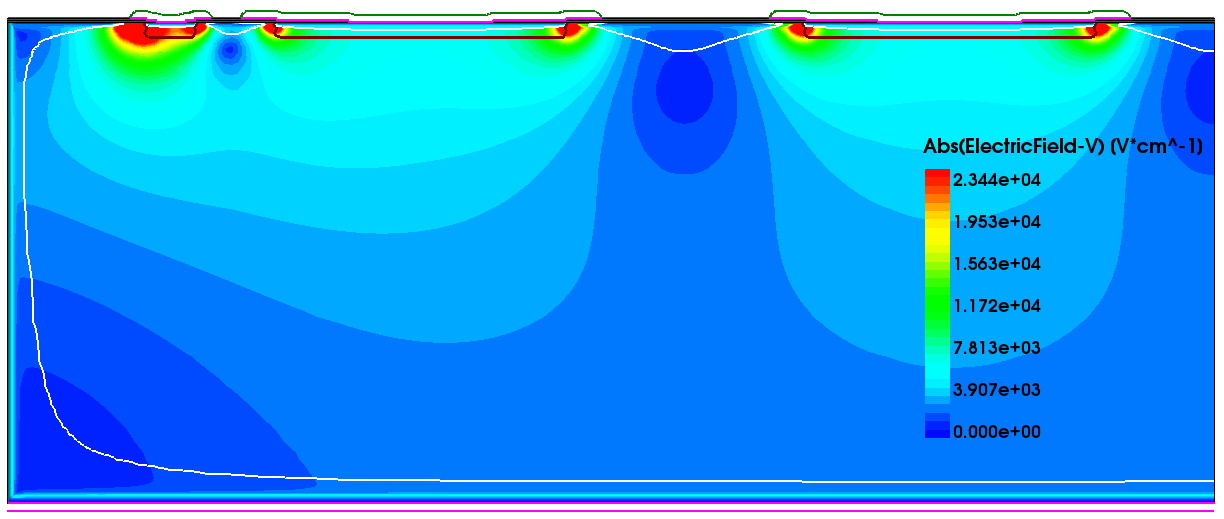
\includegraphics[width=\textwidth]{figures/ActiveEdge/Efield_28_GNDGR.png}
    \caption{28-GNDGR}
  \end{subfigure}\hfill
  \begin{subfigure}[b]{0.5\linewidth}
    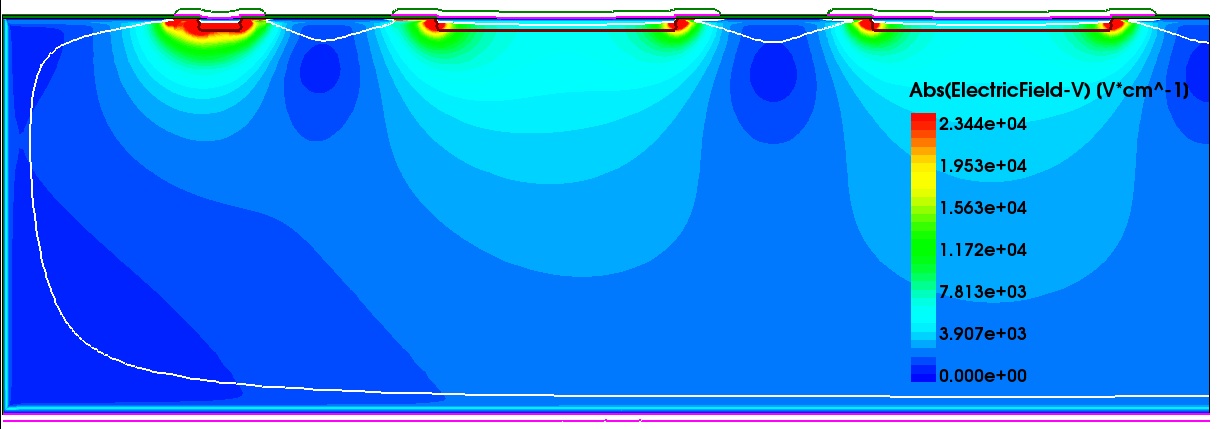
\includegraphics[width=\textwidth]{figures/ActiveEdge/Efield_55_GNDGR.png}
    \caption{55-GNDGR}
  \end{subfigure} \\
  \begin{subfigure}[b]{0.5\linewidth}
    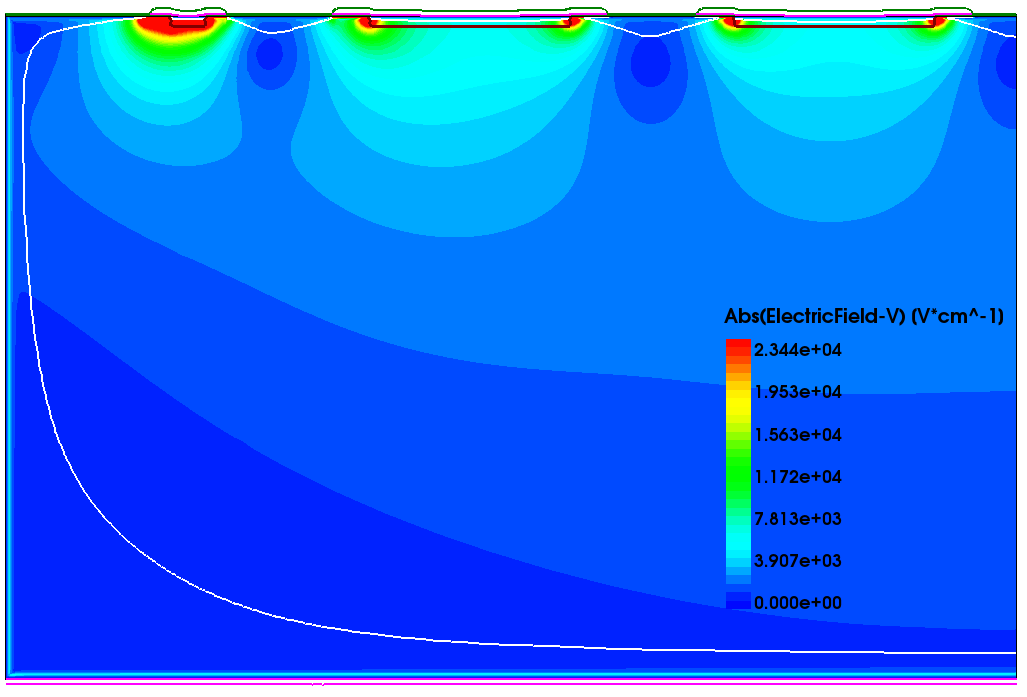
\includegraphics[width=\textwidth]{figures/ActiveEdge/Efield_55_GNDGR_100.png}
    \caption{55-GNDGR-100}
  \end{subfigure}\hfill
  \begin{subfigure}[b]{0.5\linewidth}
    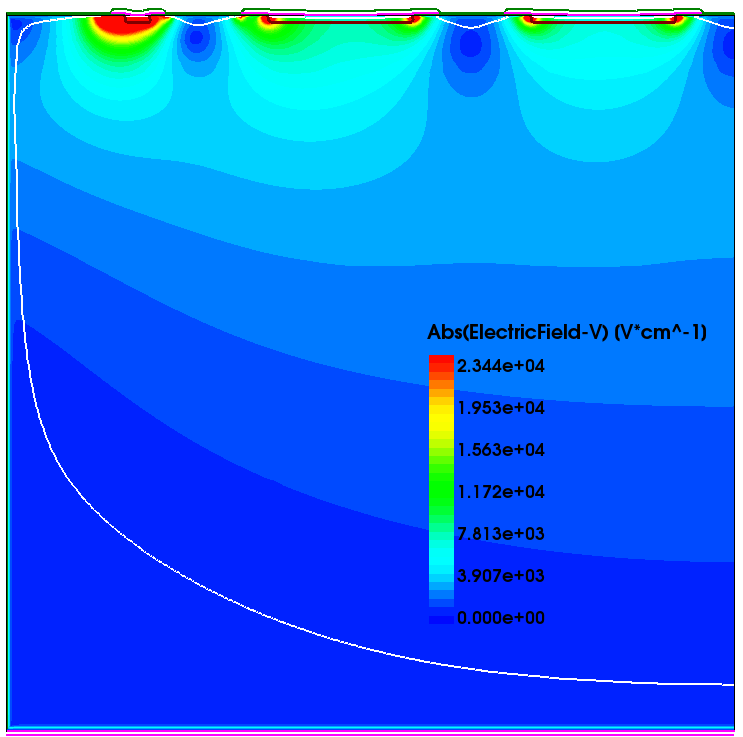
\includegraphics[width=\textwidth]{figures/ActiveEdge/Efield_55_GNDGR_150.png}
    \caption{55-GNDGR-150}
  \end{subfigure}
  \caption{Electric field distribution in TCAD simulations.}
  \label{fig:TCAD_Efield2D}
\end{figure}

The electric field and the electrostatic potential in TCAD simulations
for a cut close to the n-implants ($0.2\,\micron$ from the sensor
surface) are shown in
\cref{fig:TCAD_Efield_EPotential_sensorSurface}. Position $0\,\micron$
corresponds to the position of the first pixel. At the surface, the
breakdown electric field is never reached for the nominal
conditions. The floating guard-ring (23-FGR) shows a better potential
transition between the edge of the sensor and the first pixel.


\begin{figure}[htbp]
  \centering
  \begin{subfigure}[b]{0.5\linewidth}
    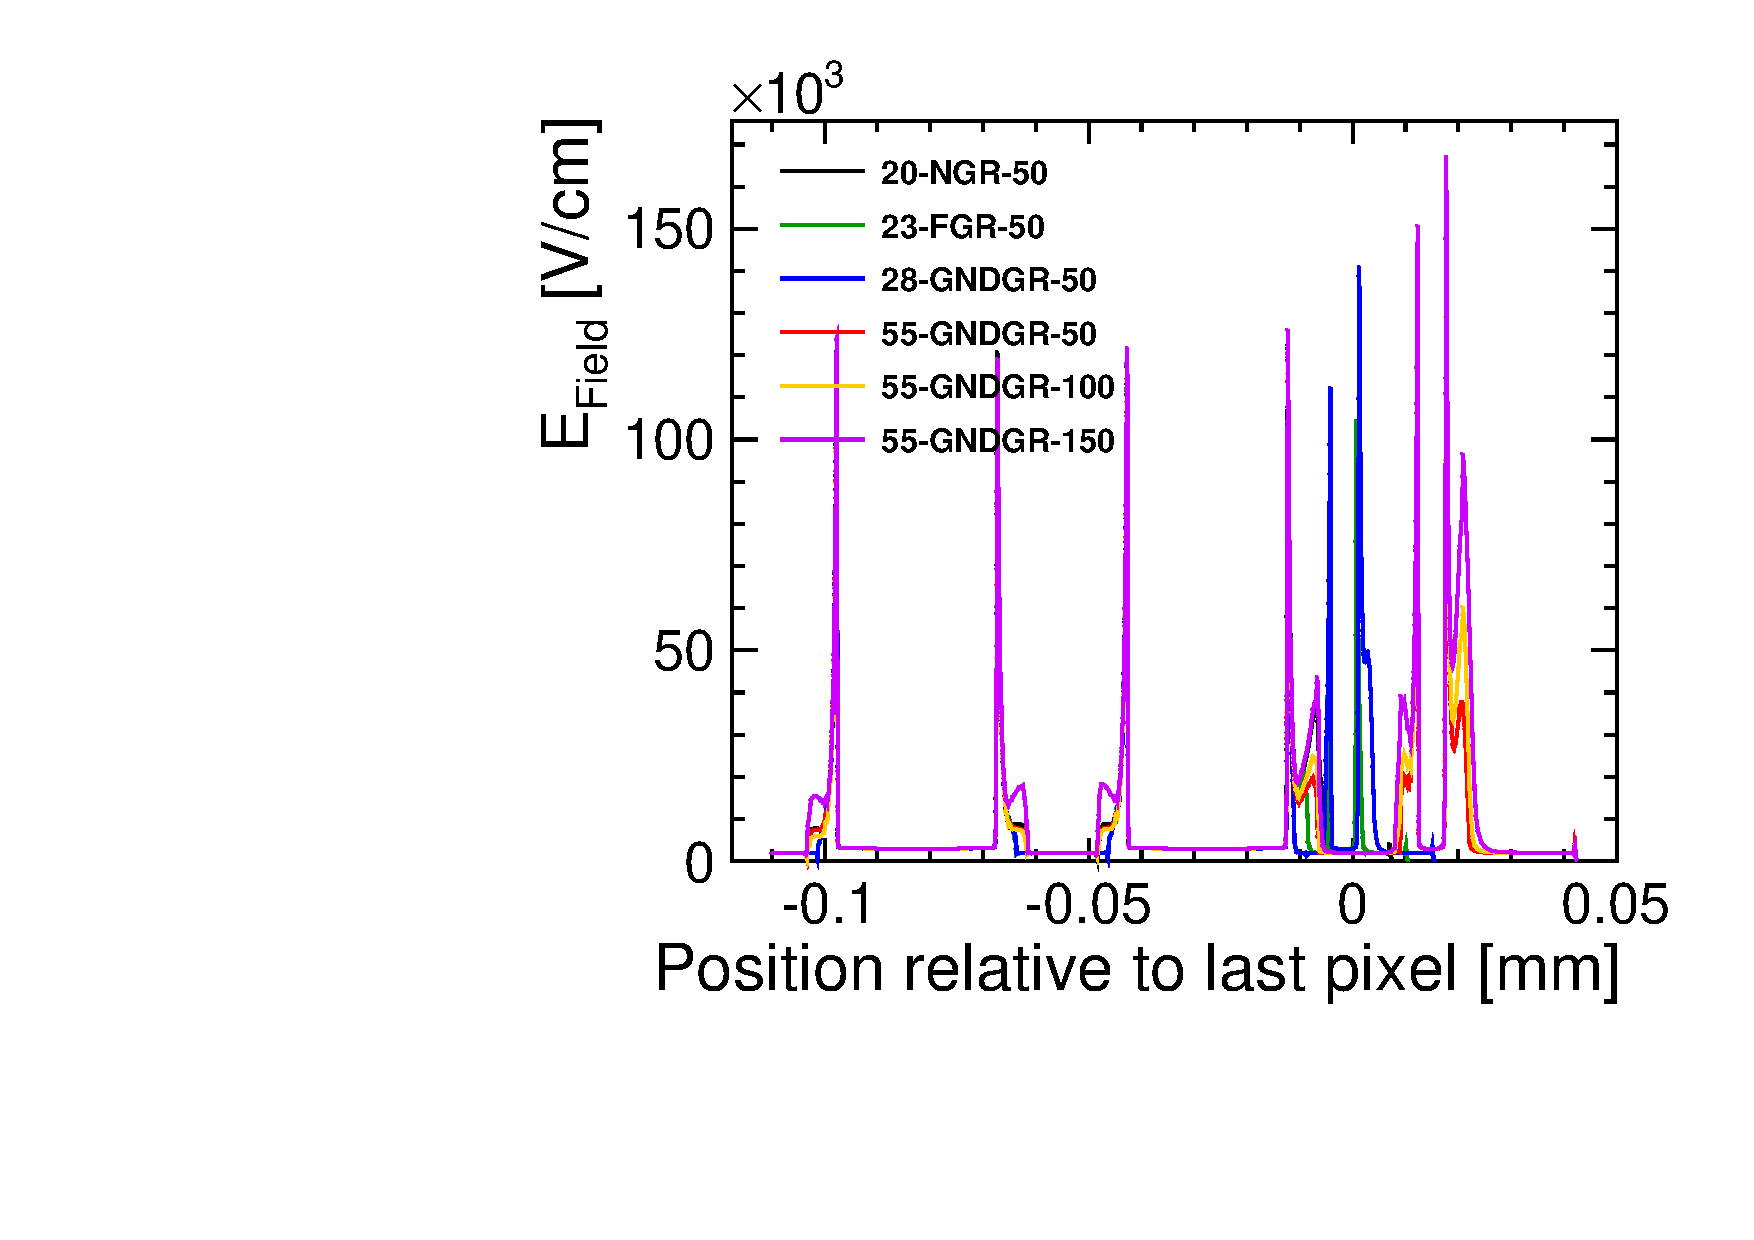
\includegraphics[width=\textwidth]{figures/ActiveEdge/Efiel_cut0_2um.pdf}
    \caption{}
  \end{subfigure}\hfill
  \begin{subfigure}[b]{0.5\linewidth}
    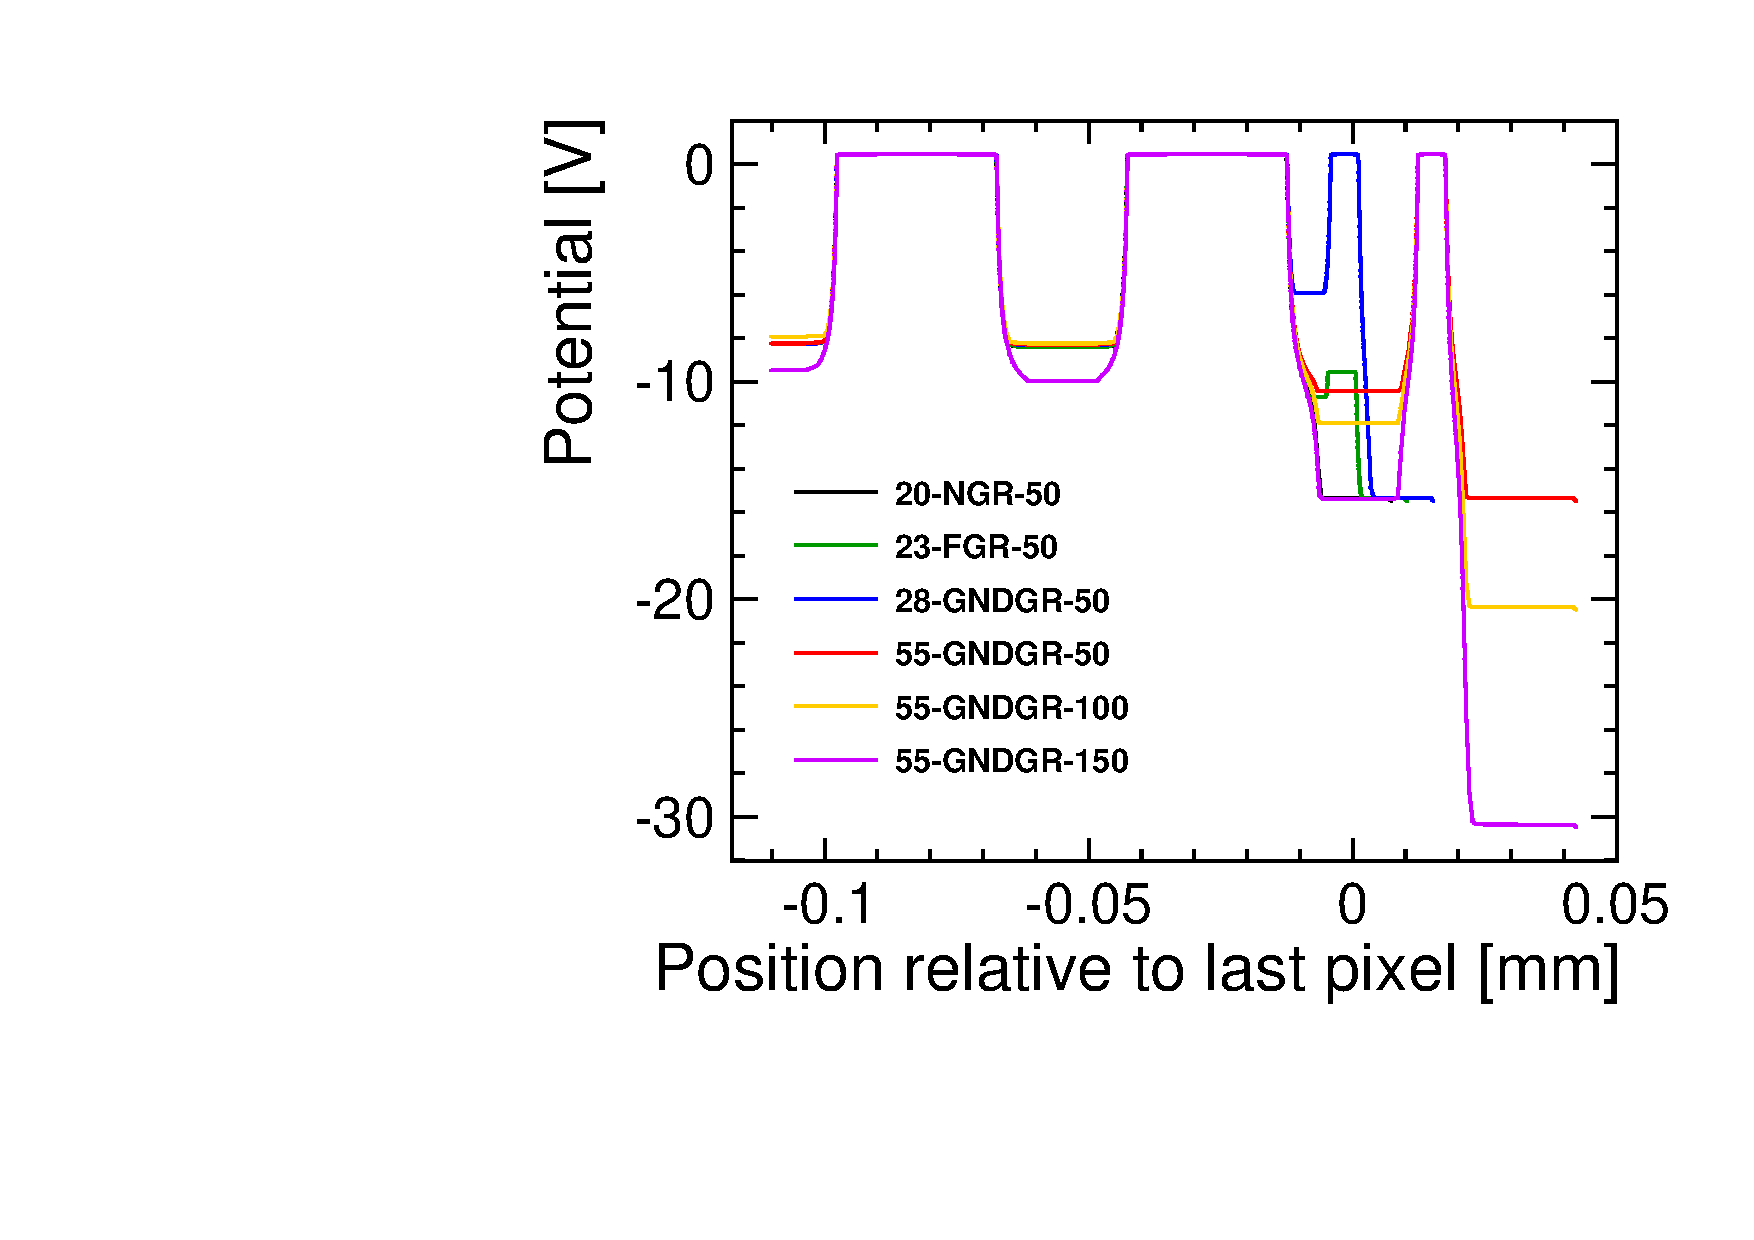
\includegraphics[width=\textwidth]{figures/ActiveEdge/EPotential_cut0_2um.pdf}
    \caption{}
  \end{subfigure}
  \caption{(a) The electric field and (b) the electrostatic potential
    at a distance of $0.2\,\micron$ from the sensor surface. Position
    $0\,\micron$ corresponds to the position of the first pixel.}
  \label{fig:TCAD_Efield_EPotential_sensorSurface}
\end{figure}

%% --------------------------------------------- %%
\subsection{Validation of simulation with data}

The transient simulation of the active edge devices is done by a
charge deposition of $10^{-5}\,\picocoulomb/\micron$ along the path of
the particle track. This corresponds to an energy deposition of
$\sim80\,\text{e-}/\micron$ as expected for the MIP in
silicon. \cref{fig:TCAD_transientSimu} illustrates a MIP traversing
the sensor at a distance of $10\,\micron$ from the left edge. The
electron density 6~ns after the particle hit is illustrated. The
electrodes collect the current generated by the electrons and it is
integrated over 15~ns.

\begin{figure}[htbp]
  \centering
  \begin{tikzpicture}
    \node[anchor=south west,inner sep=0] (image) at
    (0,0){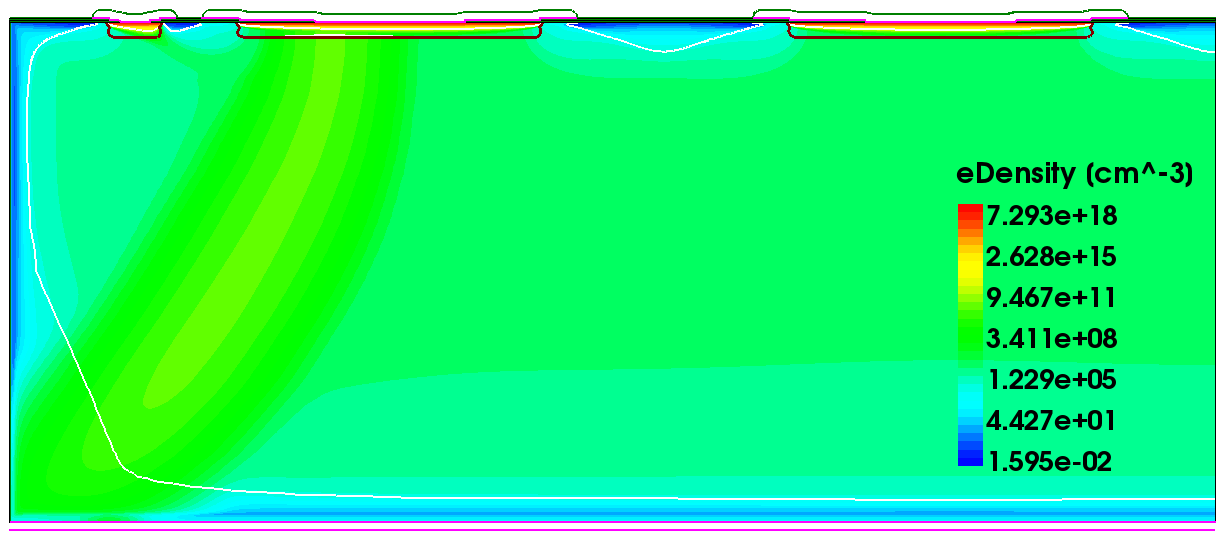
\includegraphics[width=0.7\textwidth]{figures/ActiveEdge/TCAD_transient_23FGR_hitpos_60.png}};
    \begin{scope}[x={(image.south east)},y={(image.north west)}]

      %% \draw[help lines,xstep=.1,ystep=.1] (0, 0) grid (1,1);
      %% \foreach \x in {0,1,...,9} { \node [anchor=north] at (\x/10,0) {0.\x}; }
      %% \foreach \y in {0,1,...,9} { \node [anchor=east] at (0,\y/10) {0.\y}; }

      \draw[-, dashed, very thick] (0.093, 0.05) -- (0.093, 0.96);
    \end{scope}
  \end{tikzpicture}
  \caption{Transient simulation of a particle track traversing the
    sensor at a distance of $10\,\micron$ from the edge (in dashed
    line). The electron density 6~ns after the particle hit is shown.}
  \label{fig:TCAD_transientSimu}
\end{figure}

% \begin{figure}[htbp]
%   \centering
%   \begin{minipage}[t]{.4\textwidth}
%     \centering
%     \vspace{0pt}
%     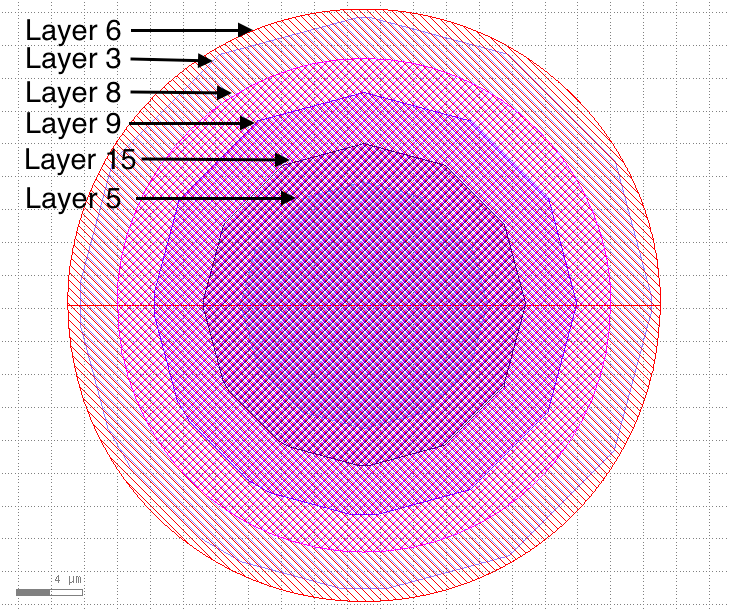
\includegraphics[width=0.95\textwidth]{figures/ActiveEdge/pixelLayout_withLayers.png}
%     \caption{}
%     \label{fig:PixelLayout}
%   \end{minipage}
%   \hfill
%   \begin{minipage}[t]{.56\textwidth}
%     \centering
%     \vspace{0pt}
%     \captionof{table}{Layers and dimensions from the gds geometry
%       (taken from Timepix 20um GR FLOAT).}
%     \label{tab:PixelStackDimensions}
%     \begin{tabular}{l c c}
%       \toprule
%       Layer number & Layer & Diameter [\micron]\\
%       \midrule
%       6 & metal & 36 \\
%       3 & - & 34.62 \\
%       8 & implant & 30 \\
%       9 & UBM (for thin film lift off metal) (??) & 25.6 \\
%       15 & passivation & 19.5 \\
%       5 & contact to connect Al to Si & 15 \\
%       \bottomrule
%     \end{tabular}
%   \end{minipage}
% \end{figure}
